\documentclass{oci}
\usepackage[utf8]{inputenc}
\usepackage{lipsum}
\usepackage{tikz}

\title{Ataque}
\codename{ataque}

\begin{document}
\begin{problemDescription}
  Ataque es un popular juego de mesa comercializado en Chile.
  El objetivo del juego es conquistar territorios para completar una misión.
  En cada turno los jugadores deben atacar un territorio enemigo quien
  intentará defenderse.

  Para poder atacar, un jugador debe lanzar una cantidad de dados de acuerdo al
  número de \emph{ejércitos} que este posea.
  Posteriormente, el jugador defensor deberá lanzar la misma cantidad de dados.
  Para saber el resultado del ataque tanto los dados del jugador atacante como
  del defensor se ordenan de mayor a menor.
  Luego, el mayor dado del atacante es comparado con el mayor dado del defensor,
  el segundo con el segundo y así en adelante.
  Notar que cada par de dados es comparado de forma independiente.
  Los jugadores pierden un ejército por cada dado en el que haya obtenido peor
  puntaje, en caso de haber empate el jugador defensor es quien sale victorioso
  y el atacante pierde un ejército.
  A continuación se muestra un ejemplo en que los jugadores lanzaron tres dados:

\begin{center}
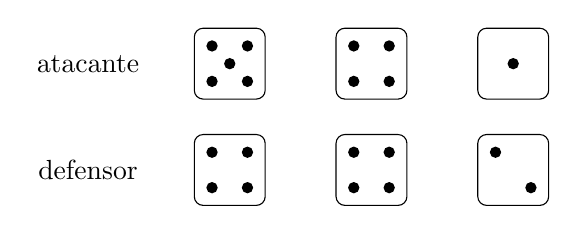
\begin{tikzpicture}[scale=.9]
\def\one{+(0.00,0.00) circle [radius=0.08]}
\def\two{+(-.25, .25) circle [radius=0.08]
	 +( .25,-.25) circle [radius=0.08]}
\def\thr{+(-.25, .25) circle [radius=0.08]
	 +(0.00,0.00) circle [radius=0.08]
	 +( .25,-.25) circle [radius=0.08]}
\def\fou{+(-.25,-.25) circle [radius=0.08]
	 +(-.25, .25) circle [radius=0.08]
	 +( .25,-.25) circle [radius=0.08]
	 +( .25, .25) circle [radius=0.08]}
\def\fiv{+(-.25,-.25) circle [radius=0.08]
	 +(-.25, .25) circle [radius=0.08]
	 +(0.00,0.00) circle [radius=0.08]
	 +( .25,-.25) circle [radius=0.08]
	 +( .25, .25) circle [radius=0.08]}
\def\six{+(-.25,-.25) circle [radius=0.08]
	 +(-.25, .25) circle [radius=0.08]
	 +(0.00,-.25) circle [radius=0.08]
	 +(0.00, .25) circle [radius=0.08]
	 +( .25,-.25) circle [radius=0.08]
	 +( .25, .25) circle [radius=0.08]}
\def\dice{
  [black,rounded corners=3.2pt]+(-.5,-.5) rectangle +(.5,.5)
}
\node at (-2, 0) {atacante};
\draw (0, 0) \dice; \fill (0, 0) \fiv;
\draw (2, 0) \dice; \fill (2, 0) \fou;
\draw (4, 0) \dice; \fill (4, 0) \one;

\node at (-2, -1.5) {defensor};
\draw (0, -1.5) \dice; \fill (0, -1.5) \fou;
\draw (2, -1.5) \dice; \fill (2, -1.5) \fou;
\draw (4, -1.5) \dice; \fill (4, -1.5) \two;
\end{tikzpicture}
\end{center}
\end{problemDescription}

\begin{inputDescription}
\lipsum[1]
\end{inputDescription}

\begin{outputDescription}
\lipsum[1]
\end{outputDescription}

\begin{scoreDescription}
  \score{10} Restricciones Subtarea1
  \score{10} Restricciones Subtarea2
  \score{10} Restricciones Subtarea3
\end{scoreDescription}

\begin{sampleDescription}
\sampleIO{sample-1}
\sampleIO{sample-2}
\end{sampleDescription}

\end{document}
